\documentclass{beamer}
\usepackage[utf8]{inputenc}

\usetheme{Madrid}
\usecolortheme{default}
\usepackage{amsmath,amssymb,amsfonts,amsthm}
\usepackage{txfonts}
\usepackage{tkz-euclide}
\usepackage{listings}
\usepackage{adjustbox}
\usepackage{array}
\usepackage{tabularx}
\usepackage{gvv}
\usepackage{lmodern}
\usepackage{circuitikz}
\usepackage{tikz}
\usepackage{graphicx}

\setbeamertemplate{page number in head/foot}[totalframenumber]

\usepackage{tcolorbox}
\tcbuselibrary{minted,breakable,xparse,skins}



\definecolor{bg}{gray}{0.95}
\DeclareTCBListing{mintedbox}{O{}m!O{}}{%
  breakable=true,
  listing engine=minted,
  listing only,
  minted language=#2,
  minted style=default,
  minted options={%
    linenos,
    gobble=0,
    breaklines=true,
    breakafter=,,
    fontsize=\small,
    numbersep=8pt,
    #1},
  boxsep=0pt,
  left skip=0pt,
  right skip=0pt,
  left=25pt,
  right=0pt,
  top=3pt,
  bottom=3pt,
  arc=5pt,
  leftrule=0pt,
  rightrule=0pt,
  bottomrule=2pt,
  toprule=2pt,
  colback=bg,
  colframe=orange!70,
  enhanced,
  overlay={%
    \begin{tcbclipinterior}
    \fill[orange!20!white] (frame.south west) rectangle ([xshift=20pt]frame.north west);
    \end{tcbclipinterior}},
  #3,
}
\lstset{
    language=C,
    basicstyle=\ttfamily\small,
    keywordstyle=\color{blue},
    stringstyle=\color{orange},
    commentstyle=\color{green!60!black},
    numbers=left,
    numberstyle=\tiny\color{gray},
    breaklines=true,
    showstringspaces=false,
}
%------------------------------------------------------------

\title
{1.6.18}
\date{August 26,2025}
\author 
{AI25BTECH11003 - Bhavesh Gaikwad}



\begin{document}


\frame{\titlepage}
\begin{frame}{Question}
\centering
Prove that points A(2,1), B(0,5) and C(-1,2) are not collinear.
\end{frame}


\begin{frame}[fragile]
    \frametitle{Theoretical Solution}
$\vec{B}-\vec{A}$=$\myvec{0-2 \\ 5-1}$ = $\myvec{-2 \\ 4}$
$\qquad \vec{C}-\vec{A}=\myvec{-1-2 \\ 2-1}$ =$\myvec{-3 \\ 1}$ \\
$\vec{M}$ = $\myvec{\vec{B}-\vec{A} & \vec{C}-\vec{A}}^T$ = $\myvec{-2 & -3 \\ 4 & 1}$\\\\

Row-reduce to compute the rank:\\

$\myvec{-2 & -3\\ 4 & 1}$ $\xrightarrow{\;R_2\leftarrow R_2+2R_1\;}$ $\myvec{-2 & -3 \\ 0 & -5}$\\

The echelon form has two nonzero rows, hence
rank(M)=2$\neq$1

\begin{align}
    \centering
    \boxed{Therefore, \, The \, points \, A(2,1), \,B(0,5) \, and \, C(-1,2) \, are \, not \, collinear.}
\end{align}
\end{frame}


\begin{frame}[fragile]
    \frametitle{Python + C Code}
    \begin{lstlisting}
#include <stdio.h>
#include <stdlib.h>
#include <math.h>
#include "libs/matfun.h"
#include "libs/geofun.h"

int main(void) {
    // Points as 2x1 column vectors
    double **A = createMat(2,1);
    double **B = createMat(2,1);
    double **C = createMat(2,1);

    // Set coordinates correctly
    A[0][0] = 2.0;  A[1][0] = 1.0;
    B[0][0] = 0.0;  B[1][0] = 5.0;
    C[0][0] = -1.0; C[1][0] = 2.0;

    // Calculate direction vectors B-A and C-A
    double **BA = Matsub(B, A, 2, 1);
    double **CA = Matsub(C, A, 2, 1);

    // Create matrix M manually as a 2x2 matrix [BA | CA]
    double **M = createMat(2, 2);
    
    // Fill M with BA and CA as columns
    M[0][0] = BA[0][0];  M[0][1] = CA[0][0];
    M[1][0] = BA[1][0];  M[1][1] = CA[1][0];

    
 \end{lstlisting}
\end{frame}


\begin{frame}[fragile]
    \frametitle{Python + C Code}
    \begin{lstlisting}
// Calculate determinant to find rank
    double det = M[0][0] * M[1][1] - M[0][1] * M[1][0];
    
    int rank;
    if (fabs(det) > 1e-10) {  // Use fabs for absolute value
        rank = 2;
    } else {
        // Check if at least one row is non-zero
        if ((fabs(M[0][0]) > 1e-10 || fabs(M[0][1]) > 1e-10) || 
            (fabs(M[1][0]) > 1e-10 || fabs(M[1][1]) > 1e-10)) {
            rank = 1;
        } else {
            rank = 0;
        }
    }

    
    \end{lstlisting}
\end{frame}

\begin{frame}[fragile]
    \frametitle{Python + C Code}
    \begin{lstlisting}
// Output result
    if (rank == 2) {
        printf("The points A, B, and C are NOT collinear (Rank = 2)\n");
    } else if (rank == 1) {
        printf("The points A, B, and C are collinear (Rank = 1)\n");
    } else {
        printf("All points coincide (Rank = 0)\n");
    }

    // Write points to .dat file
    FILE *f = fopen("points.dat", "w");
    if (f == NULL) {
        printf("Error opening file!\n");
        return 1;
    }
\end{lstlisting}
\end{frame}

\begin{frame}[fragile]
    \frametitle{Python + C Code}
    \begin{lstlisting}
   
    fprintf(f, "%.6f\t%.6f\n", A[0][0], A[1][0]);
    fprintf(f, "%.6f\t%.6f\n", B[0][0], B[1][0]);
    fprintf(f, "%.6f\t%.6f\n", C[0][0], C[1][0]);
    fclose(f);

    printf("Points written to points.dat\n");

    // Free memory
    freeMat(A, 2);
    freeMat(B, 2);
    freeMat(C, 2);
    freeMat(BA, 2);
    freeMat(CA, 2);
    freeMat(M, 2);

    return 0;
}
    \end{lstlisting}
\end{frame}

\begin{frame}[fragile]
    \frametitle{Python + C Code}
    \begin{lstlisting}
import matplotlib.pyplot as plt
import numpy as np

# Read the points from points.dat
points = []
with open("points.dat") as f:
    for line in f:
        x, y = map(float, line.split())
        points.append((x, y))

# Labels and colors for each point
labels = ['A(2,1)', 'B(0,5)', 'C(-1,2)']
colors = ['blue', 'orange', 'green']

plt.figure(figsize=(6, 6))
    \end{lstlisting}
\end{frame}

\begin{frame}[fragile]
    \frametitle{Python + C Code}
    \begin{lstlisting}
# Plot points and annotate
for (x, y), label, color in zip(points, labels, colors):
    plt.scatter(x, y, color=color, s=100, zorder=5)
    plt.text(x + 0.1, y + 0.1, label, fontsize=12, fontweight='bold')

# Draw dashed lines between B to A and C to A
# Assuming order in points.dat is A, B, C
A, B, C = points
plt.plot([B[0], A[0]], [B[1], A[1]], '--', color='gray', alpha=0.7, linewidth=1.5)
plt.plot([C[0], A[0]], [C[1], A[1]], '--', color='gray', alpha=0.7, linewidth=1.5)

    \end{lstlisting}
\end{frame}

\begin{frame}[fragile]
    \frametitle{Python + C Code}
    \begin{lstlisting}
# Grid, axes, and ticks
plt.grid(True, alpha=0.4, linestyle=':')
plt.axhline(0, color='black', linewidth=1)
plt.axvline(0, color='black', linewidth=1)
plt.xlim(-2, 4)
plt.ylim(0, 7)
plt.xticks(np.arange(-2, 5, 1))
plt.yticks(np.arange(0, 8, 1))
# Title only
plt.title('Points A, B, C', fontsize=14, fontweight='bold', pad=20)
# Remove axis labels
plt.xlabel('')
plt.ylabel('')
# Save the figure
plt.savefig('fig1.png', dpi=150, bbox_inches='tight')
plt.close()
    \end{lstlisting}
\end{frame}


\begin{frame}[fragile]
    \frametitle{Python Code}
    \begin{lstlisting}
# Code by GVV Sharma
# September 12, 2023
# Revised July 21, 2024
# released under GNU GPL

# Point Vectors
import sys                                          # for path to external scripts
sys.path.insert(0, '/home/bhavesh-g/Documents/matgeo/1.6.18/codes/line')  # path to my scripts

import numpy as np
import numpy.linalg as LA
import matplotlib.pyplot as plt
import matplotlib.image as mpimg

    \end{lstlisting}
\end{frame}

\begin{frame}[fragile]
    \frametitle{Python Code}
    \begin{lstlisting}
# local imports
from line.funcs import *
from triangle.funcs import *
from conics.funcs import circ_gen

# --- Using given points directly ---
A = np.array(([2, 1])).reshape(-1, 1)     # A(2,1)
B = np.array(([0, 5])).reshape(-1, 1)     # B(0,5)
C = np.array(([-1, 2])).reshape(-1, 1)    # C(-1,2)

# Generating all lines
x_AB = line_gen(A, B)
x_BC = line_gen(B, C)
x_CA = line_gen(C, A)

    \end{lstlisting}
\end{frame}

\begin{frame}[fragile]
    \frametitle{Python Code}
    \begin{lstlisting}
# Plotting all lines
plt.plot(x_AB[0, :], x_AB[1, :], label='$AB$')
plt.plot(x_BC[0, :], x_BC[1, :], label='$BC$')
plt.plot(x_CA[0, :], x_CA[1, :], label='$CA$')

# Labeling the coordinates
colors = np.arange(1, 4)
tri_coords = np.block([[A, B, C]])
plt.scatter(tri_coords[0, :], tri_coords[1, :], c=colors)
vert_labels = ['A', 'B', 'C']
for i, txt in enumerate(vert_labels):
    plt.annotate(
        f'{txt}\n({tri_coords[0,i]:.2f}, {tri_coords[1,i]:.2f})',
        (tri_coords[0, i], tri_coords[1, i]),
        textcoords="offset points",
        xytext=(25, 5),
        ha='center'
    )
    \end{lstlisting}
\end{frame}

\begin{frame}[fragile]
\frametitle{Python Code}
\begin{lstlisting}
# Axes crossing at origin
ax = plt.gca()
ax.spines['top'].set_color('none')
ax.spines['right'].set_color('none')
ax.spines['left'].set_position('zero')
ax.spines['bottom'].set_position('zero')

plt.grid()
plt.axis('equal')

# if using termux
plt.savefig('fig1.png')
# subprocess.run(shlex.split("termux-open fig1.pdf"))  # uncomment on Termux
# else
# plt.show()
\end{lstlisting}
    
\end{frame}

\begin{frame}{Graph}
   \centering
    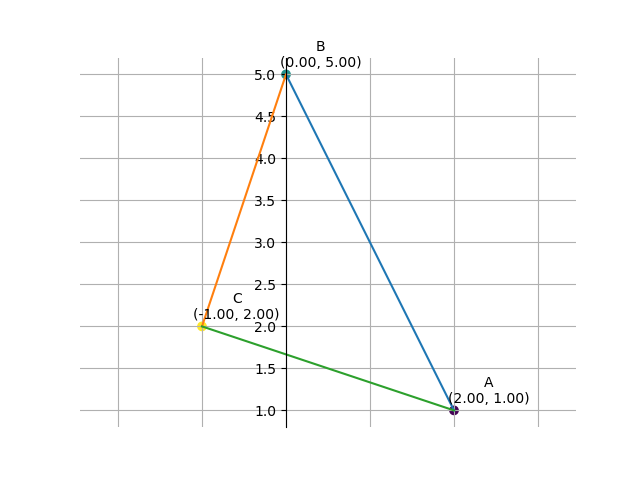
\includegraphics[width=\columnwidth, height=0.8\textheight, keepaspectratio]{figs/fig1.png}
    \label{fig:Beamer/figs/fig1.png}
\end{frame}


\end{document}